\thispagestyle{endchapter}

\begin{tcolorbox}
\vspace{80pt}

\lettrine{I}{n} the \passage{Vrtnarija} system (5.70 km/802 m at beginning of expo) we
installed a camp at --254 m in an until now torturous parallel shaft
series (\passage{Captain Kangaroo}). This was the major factor that enabled
us to add 225 m of depth to the \passage{Dark Tranquillity} series,
connecting two wings of \passage{Vrtnarija} and creating a stunning 562 m
deep alpine exchange trip. In addition we performed three major climbs
in the area of the camp in an attempt to connect \passage{Vrtnarija} to
\passage{Sistem Migovec} (11.52 km, 970 m deep), pushed \passage{Tolminska Korita}
(below the main pitch series in \passage{Vrtnarija} at -550 m) a further
--45 m, and pushed upstream above the \passage{Red Cow} sump at -750 m to
discover an aven fed watershed and an active pitch series. We now have
five major leads all at a depth greater than 500 m - two large phreatics separated by 120 m and heading in opposite
directions (\passage{Leopard} -539 m, \passage{Muddy Window} -529 m), two
large active pitch series (\passage{Tolminska Korita} -585 m, \passage{Republika}
-737 m) and the rather tight \passage{Falls Road} (-577 m).

In \passage{Captain Kangaroo} we have the \passage{Ride the
Lightning} pitch to drop, as well as a multitude of narrow rifts which
require expansion to pass at -190 to -270 m.

In the \passage{M2} part of \passage{Sistem Migovec}, progress was slower but an
aided climb was made to a phreatic series that terminates in a drafting
boulder pile, and now forms the closest approach between the two
systems.

In all, we discovered 854 m of new passage in \passage{Vrtnarija} (bringing
the total polygon length to 6.58 km) and 101 m in smaller caves and digs
on the surface, bringing the total for Migovec to 22.9 km. An updated
survey of \passage{Vrtnarija} (in extended elevation) has been prepared,
including transformation of all mountain survey data into grid north.

A slideshow presentation was given
at the end of the expedition in the Tolmin library by Andrej Fratnik
(JSPDT) and Jarvist Frost (ICCC), translated to Slovene by Jana Čarga
(JSPDT/ICCC). Our findings were also presented as a lecture at the BCRA
2009 conference by Jarvist Frost.

\end{tcolorbox}
	\backgroundsetup{	scale=1.1,
        color=black,
        opacity=1,
        angle=0,
        contents={%
                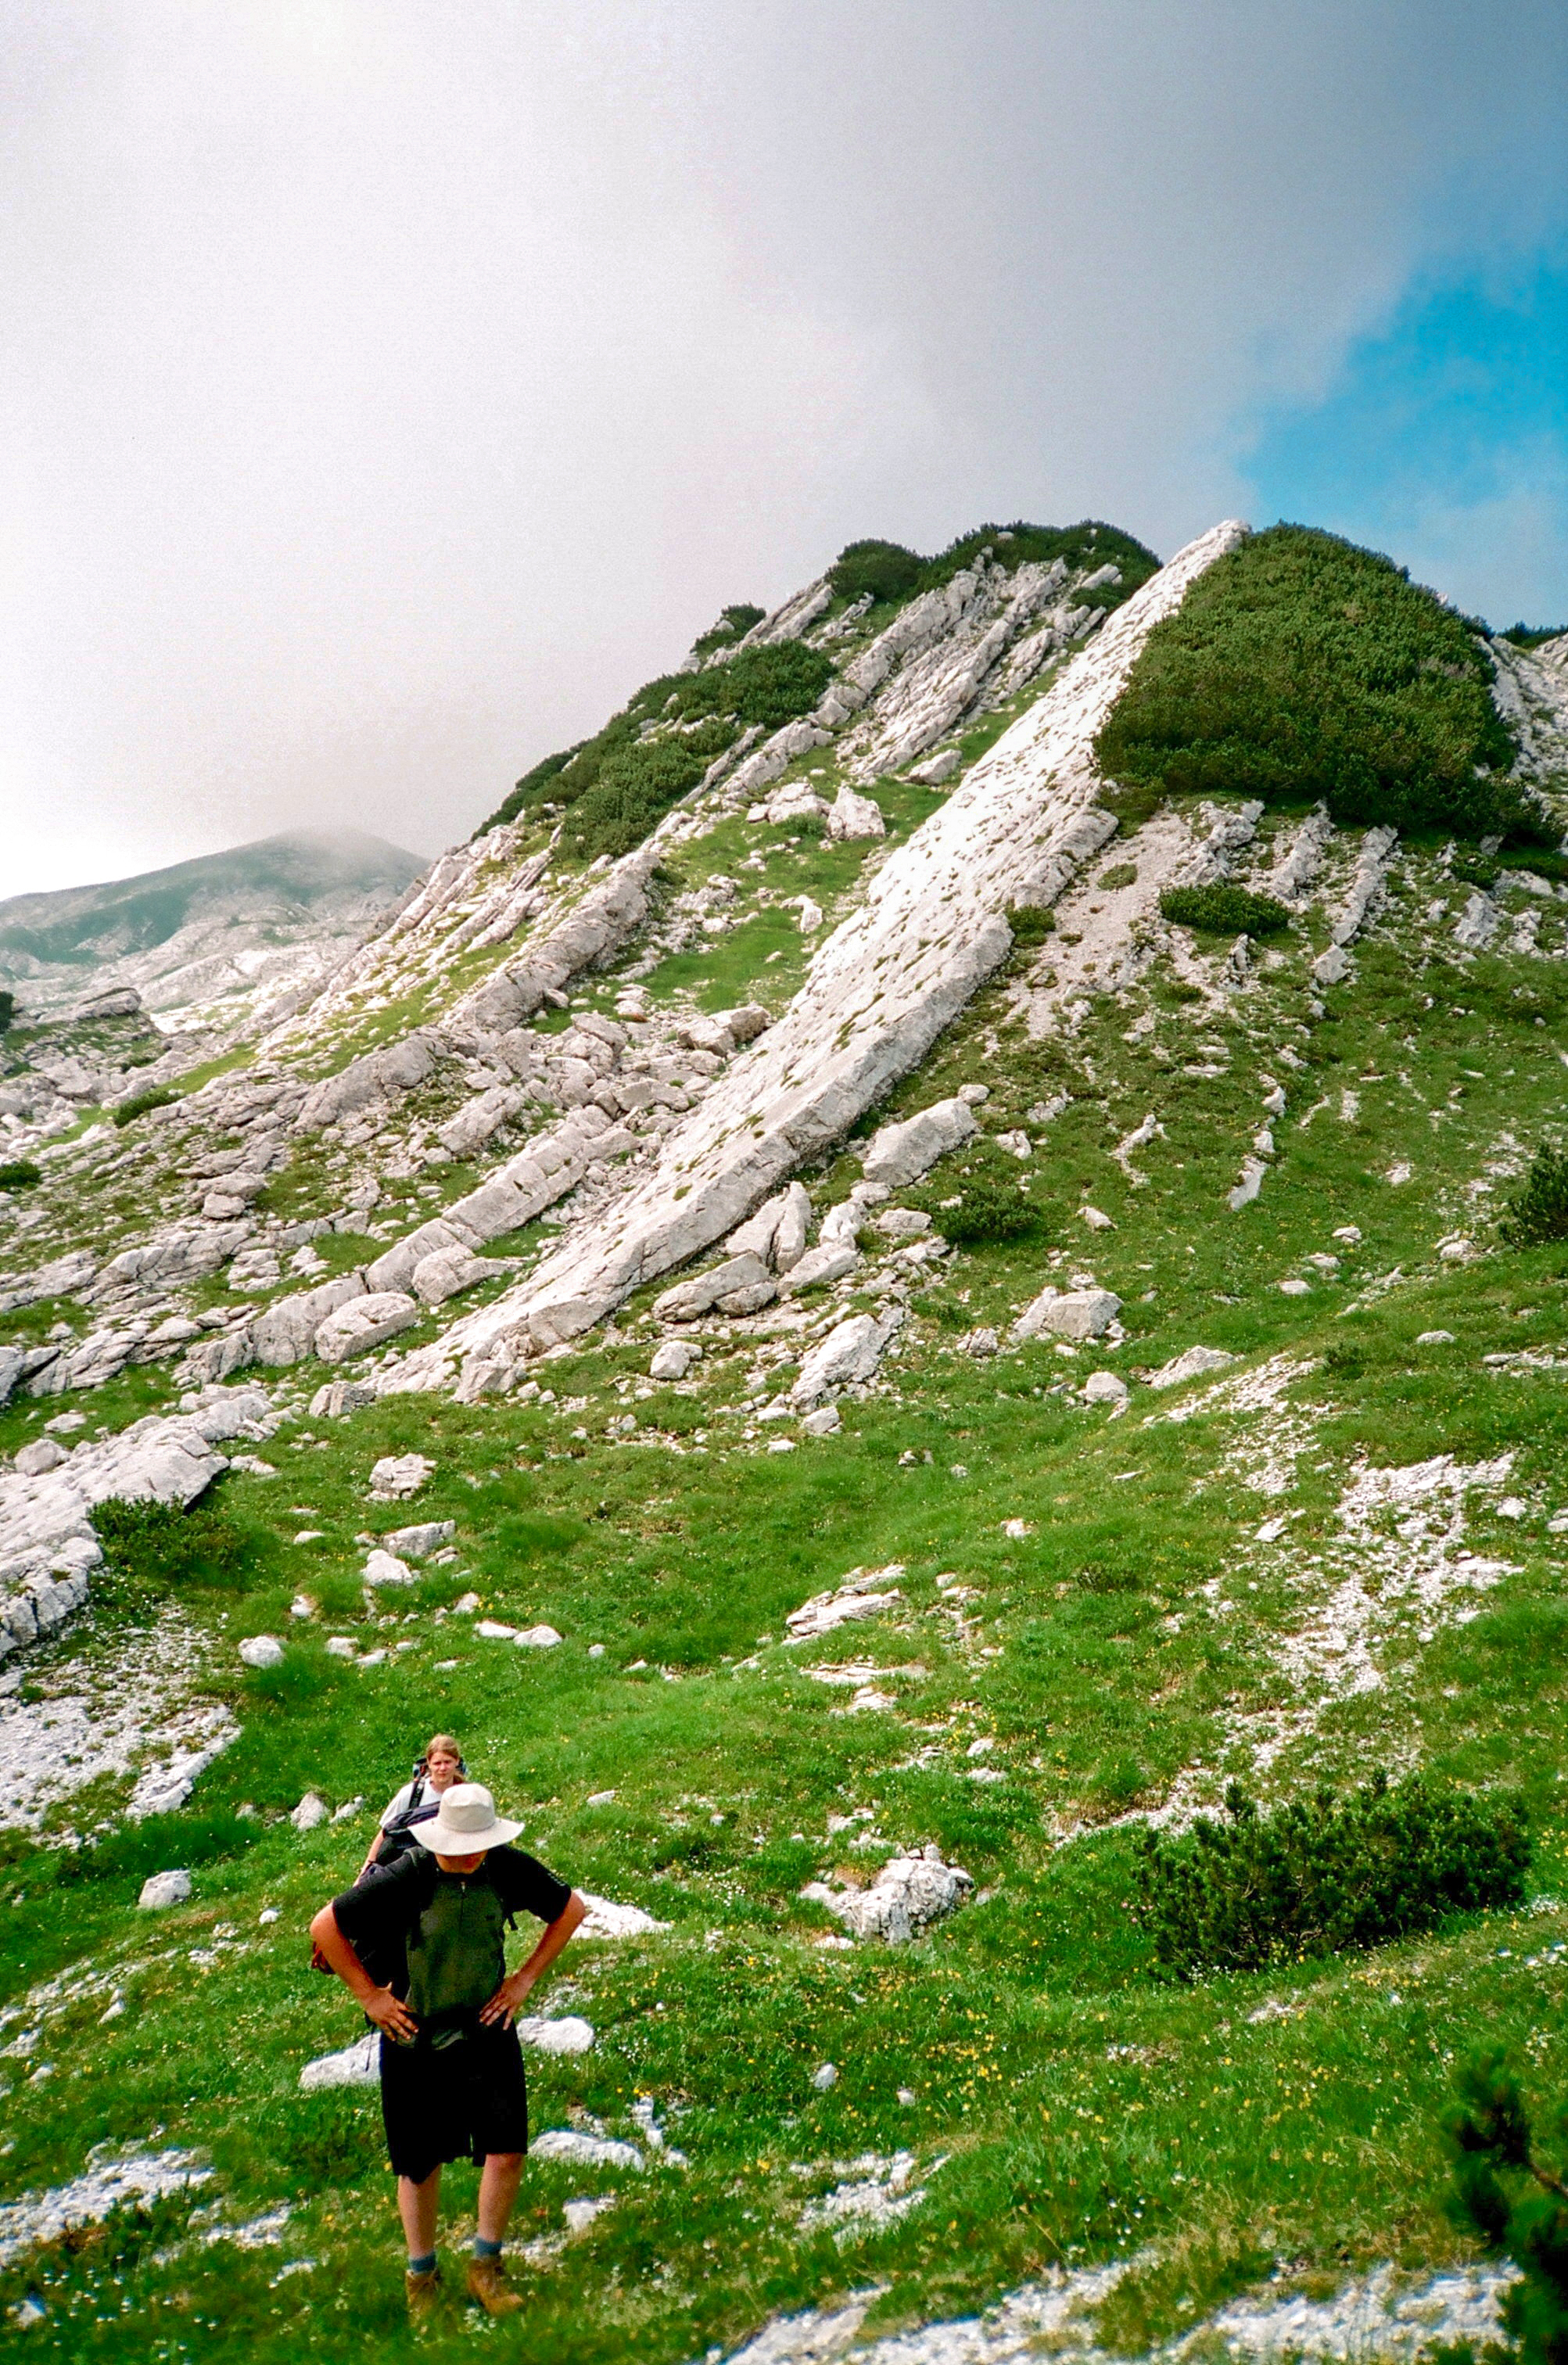
\includegraphics[height=\paperheight]{2009/outro/jarvist frost - olympus xa - superia 100 - william and alex walking past whale bone--orig.jpg}
        }
	}
\BgThispage
